\begin{anexosenv}

\partanexos

\chapter{Primeiro Anexo}

\section{Código do sistema}

O Código também pode ser acessado em

\begin{figure}[h]
	\centering
	\label{fig:codigo_pt01}
		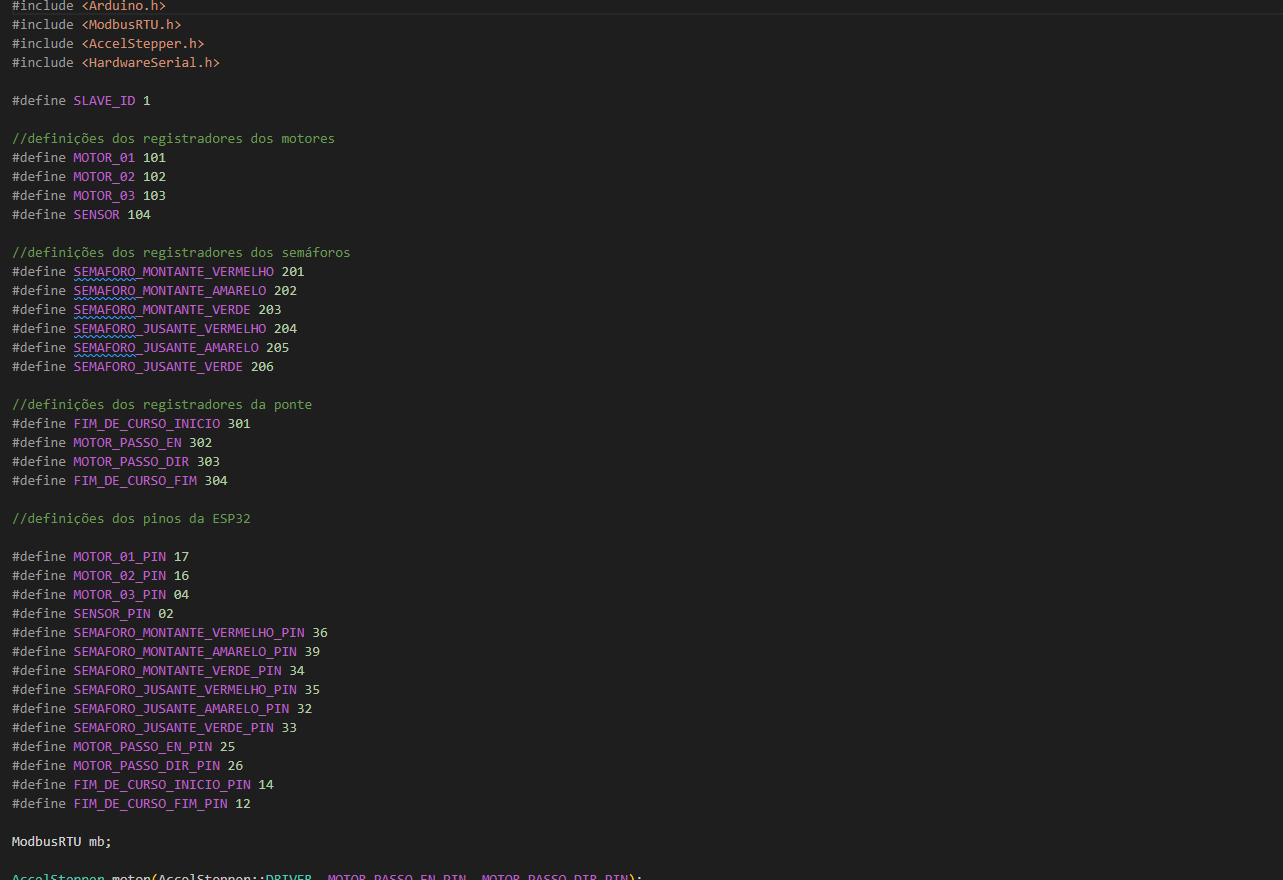
\includegraphics[keepaspectratio=true,scale=0.6]{figuras/codigo_pt1.png}
	\caption{includes)}
\end{figure}

\begin{figure}[h]
	\centering
	\label{fig:codigo_pt02}
		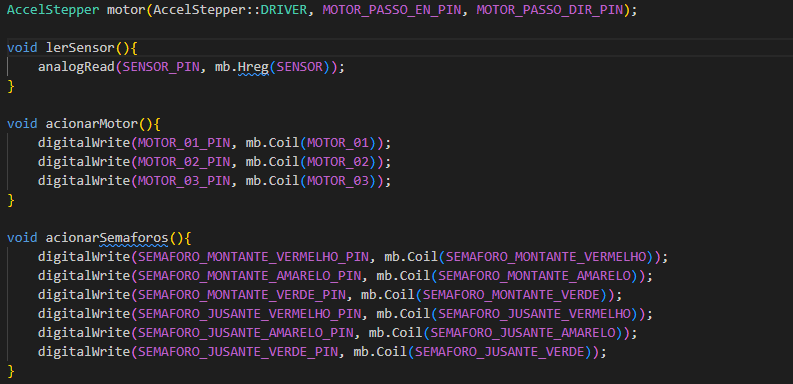
\includegraphics[keepaspectratio=true,scale=0.6]{figuras/codigo_pt2.png}
	\caption{construtor do Motor de passo e funções dos poços e semáforos)}
\end{figure}

\begin{figure}[h]
	\centering
	\label{fig:codigo_pt03}
		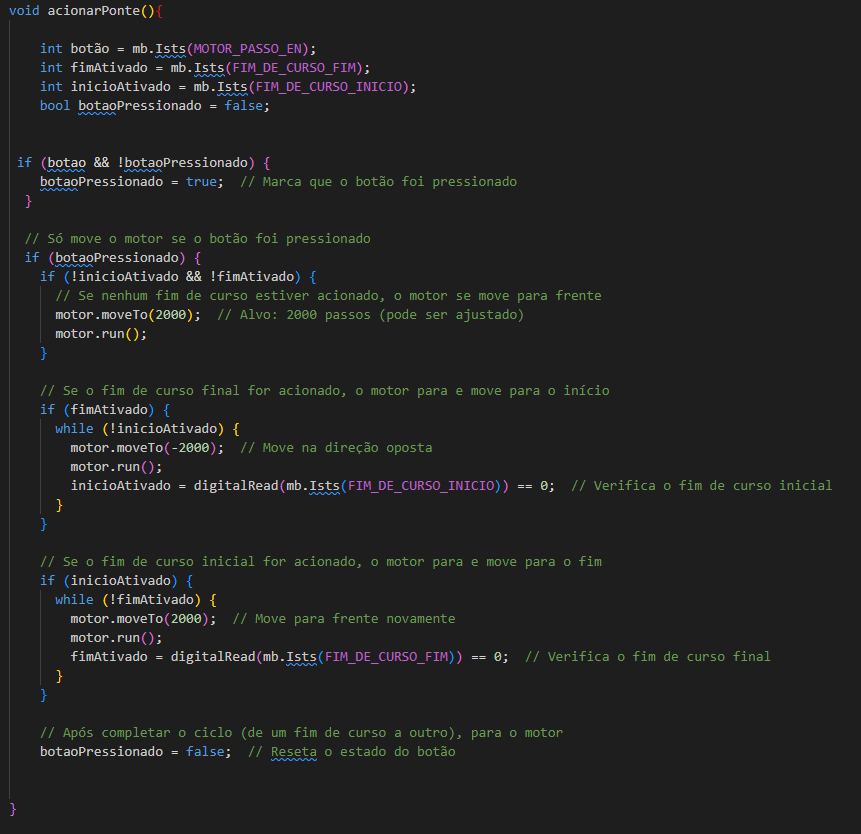
\includegraphics[keepaspectratio=true,scale=0.6]{figuras/codigo_pt3.png}
	\caption{Função de movimento do motor da ponte)}
\end{figure}

\begin{figure}[h]
	\centering
	\label{fig:codigo_pt04}
		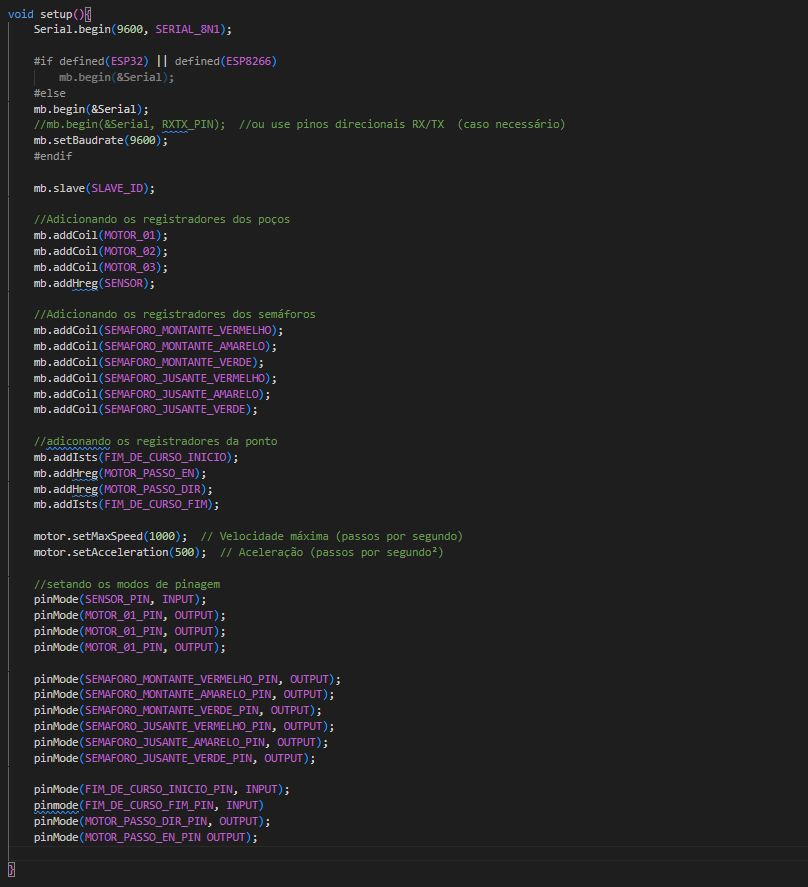
\includegraphics[keepaspectratio=true,scale=0.6]{figuras/codigo_pt4.png}
	\caption{Setup)}
\end{figure}
\begin{figure}[h]
	\centering
	\label{fig:codigo_pt05}
		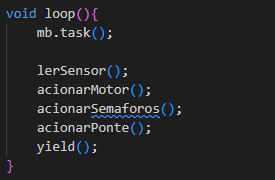
\includegraphics[keepaspectratio=true,scale=0.6]{figuras/codigo_pt5.png}
	\caption{loop principal)}
\end{figure}


\chapter{Segundo Anexo}

\section{Instalação do supervisório SCADABR}

O SCADA BR é um sistema de supervisão e controle amplamente utilizado em automação industrial e monitoramento de processos. Uma instalação adequada é essencial para garantir o funcionamento eficiente e seguro do sistema. Neste documento, detalharemos o processo de instalação do SCADA BR, abordando desde a configuração do ambiente necessário até a resolução de problemas comuns.

Para assegurar um desempenho satisfatório do SCADA BR, é fundamental que o sistema atenda aos requisitos mínimos de hardware descritos na documentação oficial \cite{scadabr_manual}. O sistema deve contar com um processador Intel Core i5 ou equivalente, 8 GB de memória RAM e pelo menos 10 GB de espaço em disco disponível para a instalação e armazenamento de dados.

Além das exigências de hardware, é necessário atender aos requisitos de software. O SCADA BR pode ser executado em sistemas operacionais como Windows 10 ou versões superiores, ou em distribuições Linux que suportem o servidor Apache Tomcat. O Java Development Kit (JDK), na versão 8 ou superior, também é um componente essencial para o funcionamento do SCADA BR. O JDK pode ser baixado diretamente do GitHub do SCADA BR, sendo recomendável escolher uma versão compatível com o sistema.

A instalação do JDK segue um processo simples. Após baixar o instalador, basta executá-lo e seguir as instruções fornecidas. Após a instalação, é necessário configurar as variáveis de ambiente, apontando para o diretório onde o JDK foi instalado e garantindo que o diretório bin do JDK esteja incluído no PATH, para que os comandos Java possam ser executados corretamente a partir do terminal. No Windows, essa configuração pode ser feita por meio do Painel de Controle, na seção de Configurações Avançadas do Sistema, dentro das Variáveis de Ambiente.

Com o JDK instalado e configurado, é possível prosseguir com a instalação do SCADA BR. Primeiramente, o arquivo compactado do SCADA BR deve ser extraído para um diretório à escolha do usuário. Em seguida, é necessário executar o arquivo de instalação, que pode ser o "setup.exe" no Windows ou o script "install.sh" no Linux. As instruções fornecidas pelo instalador guiarão o processo até a sua conclusão.

Um dos componentes essenciais para o funcionamento do SCADA BR é o banco de dados, utilizado para armazenar informações e configurações. MySQL e PostgreSQL são as opções mais recomendadas. Caso o banco de dados ainda não esteja instalado, será necessário instalá-lo e criar um banco de dados específico, junto com um usuário com as permissões adequadas. Após essa configuração inicial, o arquivo de configuração do SCADA BR, geralmente localizado no diretório "config/application.properties", deve ser editado para incluir as informações referentes ao banco de dados.

Com o SCADA BR instalado, algumas configurações adicionais podem ser necessárias, como a definição da porta de comunicação que será utilizada para a integração com outros sistemas e a configuração de usuários e permissões, o que pode ser feito através da interface administrativa do SCADA BR.

Após a conclusão dessas etapas, é possível testar a instalação acessando o sistema por meio de um navegador web, utilizando o endereço "http://localhost:8080" ou a URL definida durante a instalação. Será necessário fazer login com as credenciais padrão ou aquelas definidas durante o processo de instalação. Para verificar se o sistema está funcionando corretamente, pode-se criar um projeto básico e adicionar um dispositivo, testando a comunicação e as funcionalidades de supervisão.

Durante a instalação e configuração, podem surgir alguns problemas comuns. Um dos erros mais frequentes é a falha na conexão com o banco de dados, que pode ser resolvida verificando se o banco de dados está ativo e se as credenciais inseridas estão corretas. Outro problema recorrente envolve a configuração de portas de comunicação, devendo-se garantir que a porta designada não esteja sendo usada por outro aplicativo e que o firewall esteja configurado para permitir a comunicação.

Em caso de dificuldades adicionais, recomenda-se consultar a documentação oficial do SCADA BR, que contém informações detalhadas e sugestões de solução de problemas. Além disso, a participação em fóruns e comunidades online pode ser uma valiosa fonte de suporte e compartilhamento de experiências.


\chapter{Terceiro Anexo}

\section{Comparativo de preços entre o uso de ferramentas abertas e ferramentas pagas}

Para realizar um comparativo, serão comparadas ferramentas comerciais utilizadas no mercado e ferramentas abertas mais utlizadas pela comunidade. para o comparativo, iremos comparar o software \textit{Elipse E3} com o SCADABR, o TIA Portal da siemens com OpenPLC/programação C++ e um CLP siemens S7 com CLPs com esp32.

O Elipse E3, um sistema SCADA comercial, pode ter um custo inicial em torno de R$ 6.000 a R$ 12.000, dependendo do número de tags e funcionalidades. Em contraste, ferramentas SCADA abertas como \textit{SCADABR} ou \textit{SCADA-LTS} são gratuitas. Embora o Elipse E3 ofereça um suporte técnico robusto e funcionalidades avançadas, soluções abertas geralmente atendem a projetos industrias, com uma curva de aprendizado maior, mas a um custo substancialmente mais baixo.

Os CLPs Siemens, como o S7-1200, custam em torno de R\$ 2500 a R\$ 2800 de acordo com cotação interna, o que é um preço elevado em comparação a plataformas de hardware abertas como a ESP32, que podem ser adquiridos por menos de 200, tendo ainda assim, controladores industriais localizados para ESP32 com preços de R\$1500 a R\$2000. 

Para programar um CLP, é necessário o custo com um software de programação. A siemens possui o TIA portal, software que programa e parametriza CLPs. O custo de uma licença gira em torno de R\$ 10000 a R\$ 15000, sendo que com ferramentas abertas, o engenheiro pode escolher entre o uso de ferramentas com a linguagem C++ ou mesmo em Ladder usando o OpenPLC.

Ainda existe outro custo, oneroso ao DNIT, que é o custo de upload do código por parte do engenheiro, que custa R\$ 40000, o que custa em média 4 meses de salario de um engenheiro pleno contratado pelo DNIT para resolver o problema de automação de uma eclusa.  

% Please add the following required packages to your document preamble:
% \usepackage{booktabs}
% \usepackage{graphicx}
\begin{table}[]
\resizebox{\textwidth}{!}{%
\begin{tabular}{@{}lllll@{}}
\toprule
\textbf{Tipo de Ferramenta}                            & \textbf{Ferramenta Paga}             & \textbf{Preço estimado (R\$)}  & \textbf{Ferramenta Grautita}                                                & \textbf{Preço Estimado (R\$)}      \\ \midrule
\multicolumn{1}{|l|}{\textbf{Programação e simulação}} & \multicolumn{1}{l|}{TIA Portal}      & \multicolumn{1}{l|}{R\$10000}  & \multicolumn{1}{l|}{OpenPLC/C++}                                            & \multicolumn{1}{l|}{Gratuito}      \\ \midrule
\multicolumn{1}{|l|}{\textbf{Supervisório}}            & \multicolumn{1}{l|}{Elipse E3}       & \multicolumn{1}{l|}{R\$6000}   & \multicolumn{1}{l|}{SCADABR}                                                & \multicolumn{1}{l|}{Gratuito}      \\ \midrule
\multicolumn{1}{|l|}{\textbf{Controlador}}             & \multicolumn{1}{l|}{Siemens S7-1200} & \multicolumn{1}{l|}{R\$ 2500}  & \multicolumn{1}{l|}{Placa Industrial c/ESP32}                               & \multicolumn{1}{l|}{R\$ 1500}      \\ \midrule
\multicolumn{1}{|l|}{\textbf{Projeto+Upload}}          & \multicolumn{1}{l|}{Via contrato}    & \multicolumn{1}{l|}{R\$ 40000} & \multicolumn{1}{l|}{Contrato de um engenheiro p/ usar ferrametas Gratuitas} & \multicolumn{1}{l|}{R\$ 10000 mês} \\ \midrule
\textbf{TOTAL}                                         &                                      & R\$ 58500                      &                                                                             & R\$ 11500                          \\ \bottomrule
\end{tabular}%
}
\caption{Comparativo de preços e funcionalidades entre ferramentas comerciais e abertas}
\end{table}

\end{anexosenv}

